\subsection{Linkages}
\begin{definition}[Graph]\label{def:linkages-2}
An ordered pair $G = (V, E)$ comprising a set $V$ of vertices or nodes together with a set $E$ of edges or lines
\end{definition} 
\begin{definition}[Linkage]\label{def:linkages-1}
A collection of fixed-length 1D segments joined at their endpoints to form a graph.
\end{definition} 
A linkage can be thought of as a type of path-connected graph, i.e. the segments of a linkage are the edges of a graph, and the endpoints of the segments are the vertices. For this paper, we restrict our self to linkages that are simple planar graphs, i.e. a linkage that:
\begin{itemize}
\item[\rn{1}] does not have multiple edges between any pair of vertices,
\item[\rn{2}] does not have edges that cross, or
\item[\rn{3}] have loops (i.e. $(v,v) \in E$).
\end{itemize}  
\begin{definition}[Cycle]\label{def:linkages-3}
 A closed walk with no repetitions of vertices or edges allowed, other than the repetition of the starting and ending vertex
\end{definition} 
\begin{definition}[Configuration]\label{def:linkages-6}
A specification of the location of all the link endpoints, link orientations and
joint angles.\cite{demaine2008geometric}
\end{definition}
\begin{definition}[Configuration Space]\label{def:linkages-7}
The space of all configurations of a linkage.
\end{definition} 
A configurations space is said to be continuous if for any two configurations, $\mathcal{A}$ and $\mathcal{B}$ of a linkage $L$, $\mathcal{A}$ can be continuously reconfigured to $\mathcal{B}$ such that, the reconfigurations reside in the configuration domain, $L$ remains rigid throughout reconfiguration (i.e. all links' lengths are preserved), and no violations of linkage intersection conditions. 
\begin{definition}[Pinned Joint]\label{def:linkages-8}
A vertex of a graph (or linkage) that is fixed to a position in a plane.
\end{definition} 
\begin{definition}[Free Joint]\label{def:linkages-8}
A vertex of a graph (or linkage) that is not fixed to a position in a plane.
\end{definition} 
\begin{figure}[h]
\begin{center}
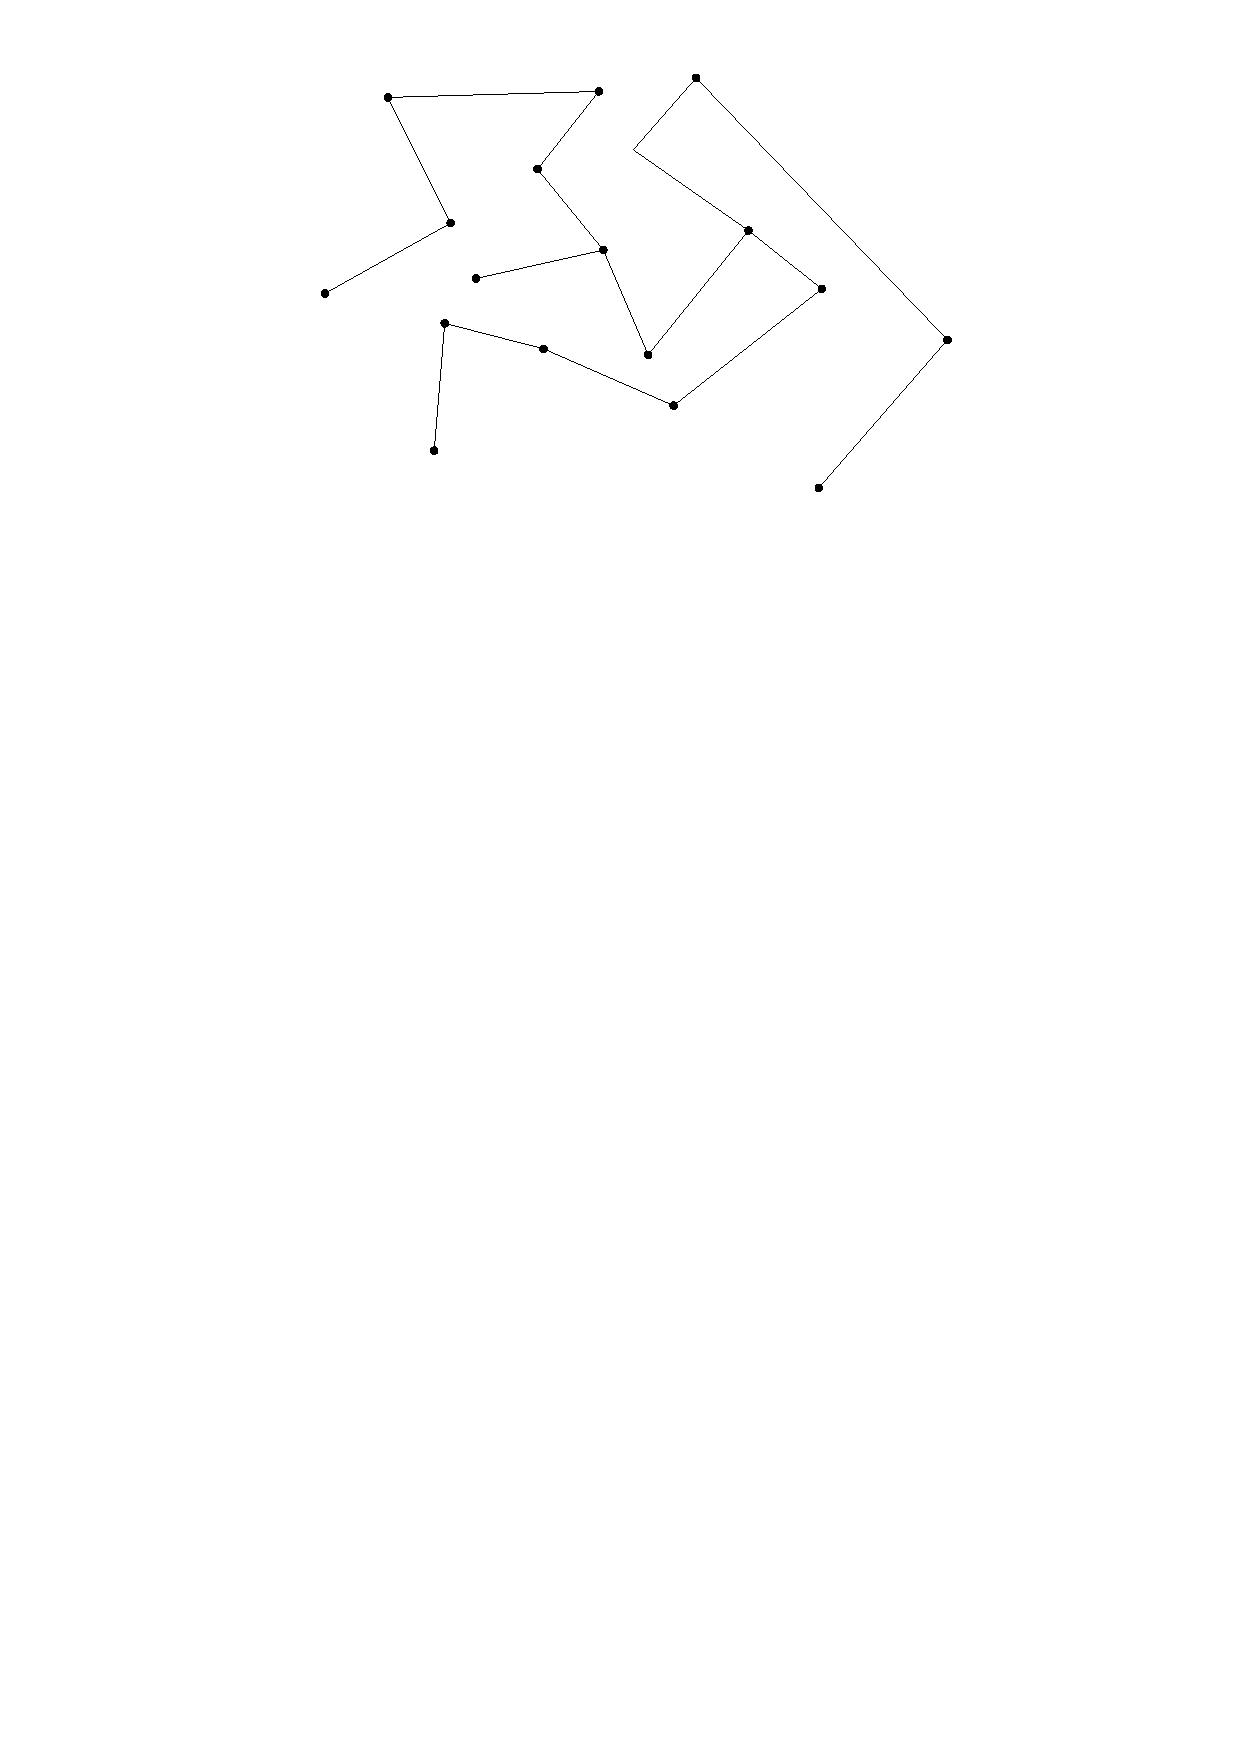
\includegraphics[scale=.5]{graphics/randomLinkage.pdf}
\end{center} 
\caption{A linkage with joints.}
\end{figure} 
\begin{figure}[h]
\begin{center}
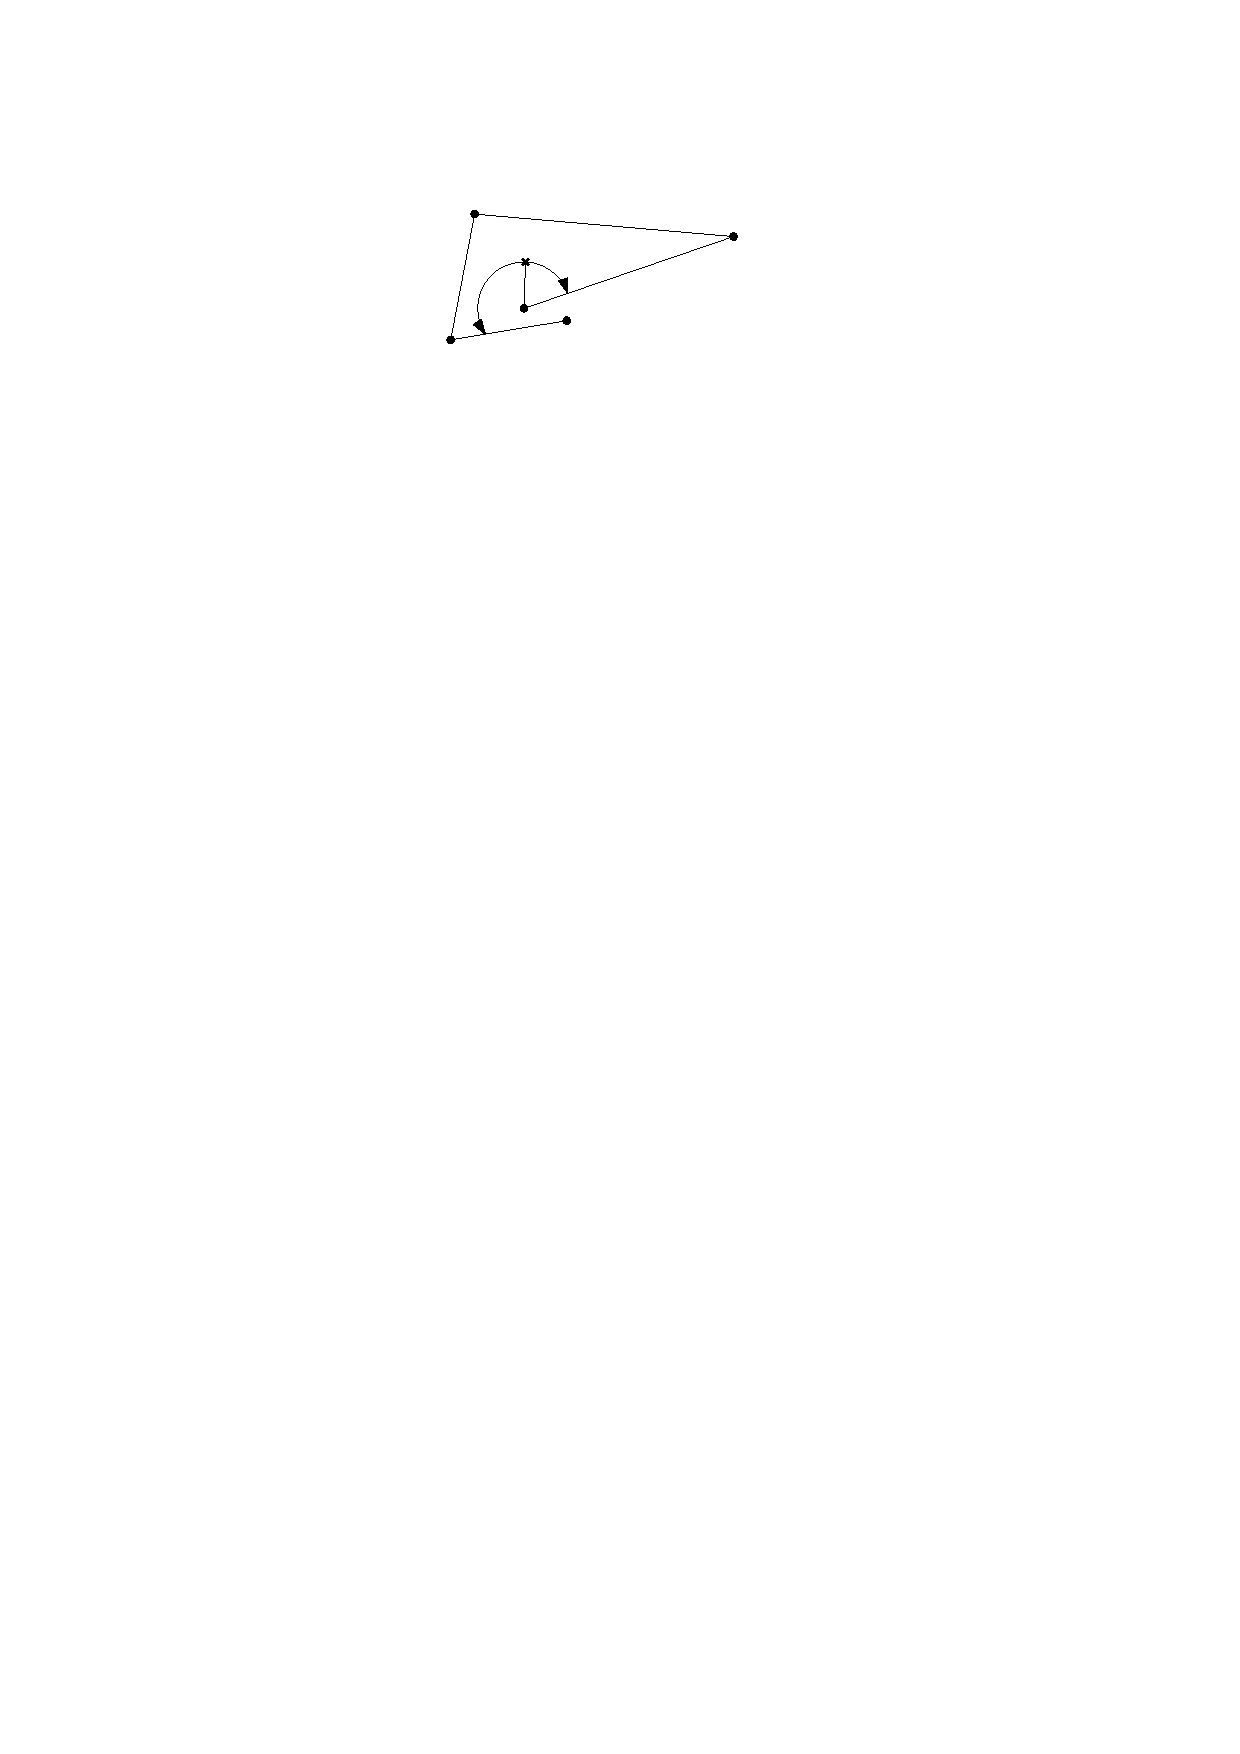
\includegraphics{graphics/freeJointPinnedJoint.pdf}
\end{center} 
\caption{The cross represents a free joint; the pinned joints are denoted as disks.  The range of motion shown by the arc describes the continous configuration space of the linkage.}
\end{figure} 

For illustrations in the remainder of this paper, free joints will be represented as crosses and pinned joints will be represented as disks.
\subsubsection{Polygonal Linkages}
\begin{figure}[!ht]
\begin{center}
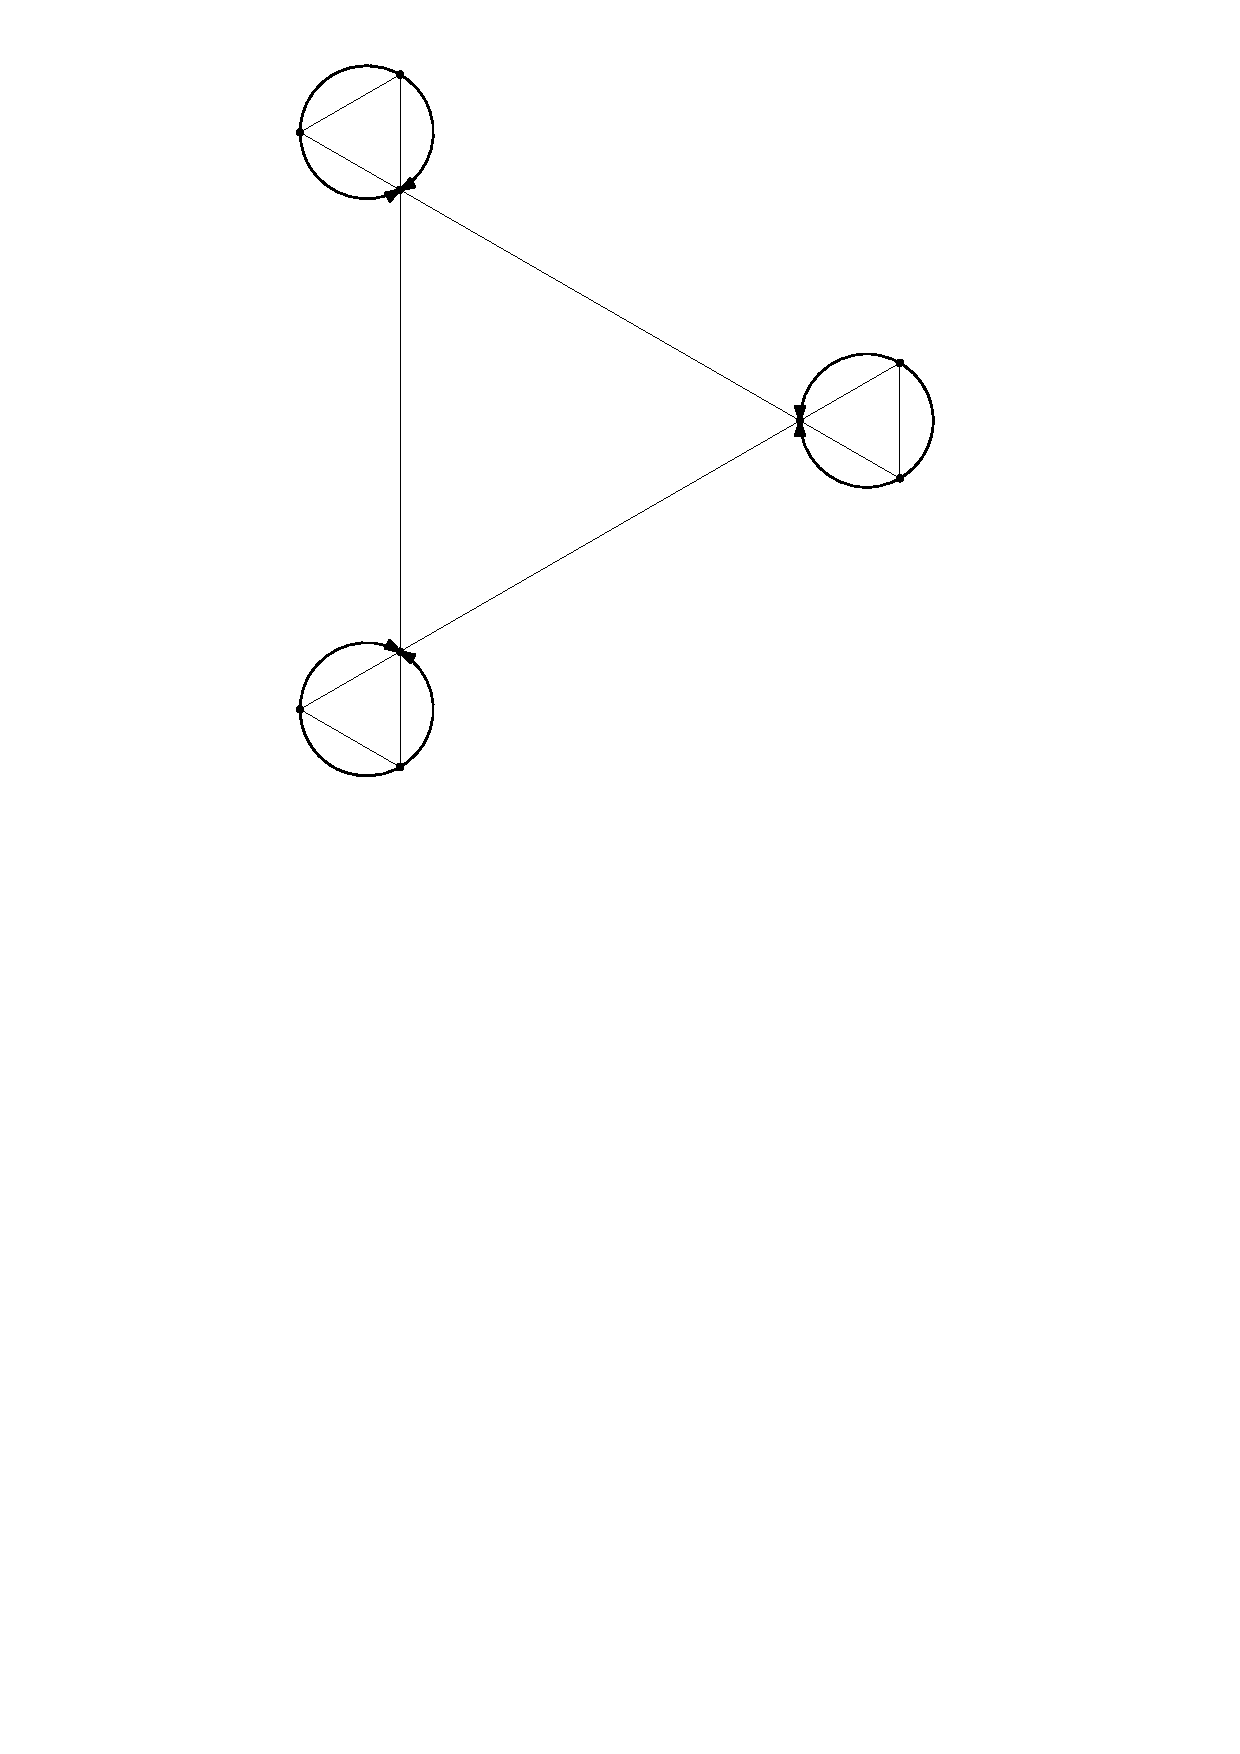
\includegraphics{graphics/PolygonalLinkageWithConfigurationSpace.pdf}
\end{center} 
\caption{\textbf{Not sure how to describe this graph with free joints, pinned joints.  Do I need to define another joint(i.e. axis of rotation joint)?}}
\end{figure} 